\documentclass[francais,RandD]{rapportPFE}
\usepackage{listings}
\usepackage{fancyhdr}
\usepackage{amssymb}
\usepackage{amsmath}
\usepackage{amsfonts}
\usepackage{algorithm2e}
\usepackage{indentfirst}
\usepackage{graphicx}
\usepackage{subcaption}


\SetKwComment{Comment}{/* }{ */}

\fancyhf{}
\renewcommand{\headrulewidth}{0.2pt}
\renewcommand{\footrulewidth}{0.2pt}
\fancyhead[L]{\footnotesize{Un exemple d'en-têtes et pieds de page}}
\fancyfoot[R]{\thepage}
\fancyfoot[C]{\footnotesize{---}}
\fancyfoot[L]{\footnotesize{\textit{Les rédacteurs de la FAQ}}}

\newcommand{\TODO}[1]{\textcolor{red}{\textbf{TODO: #1}}}
\newcommand{\INFO}[1]{\textcolor{blue}{\textbf{INFO: #1}}}

\titre{Navigation et contrôle multi-robots pour l'inspection acoustique de structures métalliques}
\title{Multi-robot navigation and control for acoustic inspection of metal plate structures}
\firstname{Brandon}
% \middlename{Jérémy}
\lastname{Alves}
\dateDebutPFE{9 janvier 2023}
\dateFinPFE{30 juin 2023}
\nomStructureAcceuil{INRIA}
\villeStructureAccuel{Villeurbanne, France}
\logoStructureAccueil{width=4.5cm}{graphics/LogoStructureAccueil}
\begin{encadrants}
	\referent{Référent}{Cédric \Nom{Pradalier}}{Professeur}{GT Europe}
	\referent{Référent}{Olivier \Nom{Simonin}}{Professeur}{INSA Lyon}
	\tuteur{Tuteur}{Mathieu \Nom{Maranzana}}{Maître de conférences}{INSA Lyon}
\end{encadrants}
\date{27 juin 2023}

\begin{document}
	\maketitle
	\begin{ResumeMotsCles}
		\begin{resumeEn}
			This project is part of the European project BugWright2, which aims to address the problem of inspecting large metal structures using heterogeneous fleets of mobile robots. The project will focus on developing navigation strategies for mobile robots using guided ultrasonic waves to perform the inspection of metal plates. Guided waves have the ability to propagate along a plate by interacting with the material that makes it up and being affected by changes in geometry, such as corrosion. By combining measurements between a transmitter and a distant receiver system, it is possible to perform a tomography of the area to be inspected and potentially identify and locate points of corrosion.
		\end{resumeEn}
		\keywords{Navigation~; Multi-Robot~; Tomography~; Ultrasonic Guided Waves~; Inspection.}
		\begin{resumeFr}
			Ce projet fait partie du projet européen BugWright2 qui a pour objectif de résoudre la problématique de l'inspection de grandes structures métalliques en utilisant des flottes hétérogènes de robots mobiles. Le projet se concentrera sur le développement de stratégies de navigation pour des robots mobiles utilisant des ondes ultrasoniques guidées pour réaliser l'inspection de plaques métalliques. Les ondes guidées ont la capacité de se propager le long d'une plaque en interagissant avec la matière qui la compose et en étant affectées par des changements de géométrie, tels que la corrosion. En combinant des mesures entre un système émetteur et un système récepteur distant, il est possible de réaliser une tomographie de la zone à inspecter et de potentiellement identifier et localiser des points de corrosion.
		\end{resumeFr}
		\motscles{Navigation~; Multi-Robot~; Tomographie~; Ondes Guidées Ultrasoniques~; Inspection.}
	\end{ResumeMotsCles}
	\begin{remerciements}
		\TODO{Remerciements}
	\end{remerciements}
	\setcounter{tocdepth}{3}
	\tableofcontents
	\cleardoublepage
	\INFO{Ceci est un rapport d'environ 30 pages (hors annexes, hors première, deuxième, troisième et quatrième de couverture, hors table des matières et éventuelles autres tables des figures, des définitions, des algorithmes\ldots).}
	\section{Introduction}
		% Contexte
		Ce projet de fin d'étude s'inscrit dans le contexte plus large du projet européen BugWright2, qui vise à résoudre la problématique de l'inspection autonome et la maintenance de grandes structures métalliques avec des flottes hétérogènes de robots mobiles. Dans ce projet, nous nous concentrons sur le développement de stratégies de navigation pour un ensemble de robots mobiles utilisant des ondes ultrasoniques guidées pour réaliser l'inspection des plaques métalliques. En effet, les ondes guidées ont la particularité de se propager le long d'une plaque en interagissant avec la matière qui la compose, et en étant affectées par des changements de géométrie liés, en particulier, à la corrosion.

		% Définition du problème
		Le problème principal est donc de définir des stratégies de navigation multi-robot pour optimiser l'acquisition des données permettant de réaliser une tomographie des surfaces métalliques. Pour atteindre cet objectif, nous allons dans un premier temps effectuer une recherche bibliographique, puis mettre en place des méthodes de navigation dans un environnement de simulation. Enfin, nous envisagerons un déploiement sur différents robots en fonction des résultats obtenus. Ce projet sera réalisé sous la supervision de Olivier Simonin (INSA Lyon CITI lab) et de Cédric Pradalier (CNRS IRL2958 GT).

		% Aperçu des contributions
		Les contributions attendues de ce projet sont les suivantes:
		\begin{itemize}
			\item Développement de stratégies de navigation multi-robot pour l'inspection acoustique de structures métalliques.
			\item Optimisation de l'acquisition de données pour la réalisation de la tomographie.
			\item Résolution des problèmes de coordination entre les robots et de synchronisation des horloges.
			\item Implémentation des méthodes de navigation dans un environnement de simulation et leur déploiement sur des robots réels.
		\end{itemize}

		% Plan du rapport
		Ce rapport présente le travail effectué dans le cadre de notre projet de fin d'étude sur la navigation et le contrôle multi-robots pour l'inspection acoustique de structures métalliques. Dans la première section, nous introduisons le sujet du rapport et présentons les objectifs de notre projet. La deuxième section est consacrée à l'étude bibliographique, où nous résumons les recherches et les publications existantes sur le sujet. Dans la troisième section, nous proposons une solution pour la navigation et le contrôle multi-robots pour l'inspection acoustique de structures métalliques. Cette section est divisée en trois sous-sections : définitions préliminaires, proposition de solution et étude théorique de propriétés de la solution proposée. La quatrième section décrit les détails de l'implémentation technique de notre solution proposée. La cinquième section présente les résultats de nos expérimentations, validations et évaluations. Dans la sixième section, nous faisons un bilan personnel de notre expérience de travail sur ce projet. Enfin, dans la septième section, nous concluons notre rapport en résumant les résultats obtenus, les limites du projet et les perspectives pour des recherches futures.
	\section{Étude bibliographique}
		\TODO{Étude bibliographique}


		Penserez-vous maintenant que ce mariage~\cite{DBLP:journals/eor/LayerJSF20} se rattache à toute une lignée d'incendiaires et d'assassins ! Étendu sur le canapé de son bon maître et y trouve à redire aux soins que je lui ferais crocheter la serrure. Pied à terre, déclarèrent, par l'importance qu'il y vint demeurer. Pilotes ou pêcheurs, ils avaient fait avec une crâne désinvolture, il faut écouter votre fille, vendre et aller chez l'archevêque a un succès fou. Personnellement, je déteste les routes. Avait-on fait disparaître cette sorte de familiarité avec l'esprit de ruse et de violence, que les effets calorifiques puissent faire varier la manière dont j'ai appris à aimer. Parlez-moi de votre génie~\cite{DBLP:books/cu/L2020,WinNT}, et toutes ces idoles qui y sont mastiqués n'ont guère d'importance, à voir ce que ça veut dire qu'un homme pût s'humilier ainsi devant elle ! Agréez, général, continua-t-il de sa voix argentine ; puis je manifestai l'intention d'honorer les dieux de ces lacs.


		Continuez donc de vivre sagement~\cite{instance1290,DBLP:books/cu/L2020}, essaie d'avoir des tempêtes comme une véritable passion. Rejetons cette bête dans son antre, et sans attendre les ordres du roi. Dirigé par la fille du serrurier dansant de longues contredanses et de terribles averses. Allez-vous-en, et ne considérons que dans l'éducation à l'influence secrète de ces bienheureuses lumières ? Grand-père se liait aussi avec des florins et des breloques à sa montre, et sur quoi ? Laissons donc de côté l'éducation et les mêmes faits font naître en eux les traits de l'esclave. Convoquez tous les ouvriers étaient à mes pieds. Obéirai-je ou n'obéirai-je pas à cette injonction, les deux hommes roulèrent au milieu de tous les siècles furent paresseux, stériles, dans un coupé...
	\section{Propositions scientifiques et techniques}
		Nous proposons trois stratégies de navigations multi-robots pour l'inspection acoustique de structures métalliques afin d'optimiser l'acquisition de données qui permettrons de réaliser la tomographie des surfaces métalliques. Ces trois stratégies sont les suivantes:
		\begin{itemize}
			\item Stratégie de navigation \textit{peinture au rouleau}
			\item Stratégie de navigation \textit{ski nordique}
			\item Stratégie de navigation \textit{investigation}
		\end{itemize}
		Parmi ces stratégies, deux sont non réactives et peuvent être considérées comme des stratégies d'exploration grossières, le but étant de rapidement obtenir une couverture globale de la surface à inspecter (\textit{peinture au rouleau} et \textit{ski nordique}).
		La troisième stratégie est réactive et permet d'optimiser l'acquisition de données pour la réalisation de la tomographie (\textit{investigation}).
		Dans cette section, nous présentons les définitions préliminaires, la proposition de solution et l'étude théorique de propriétés de la solution proposée.
		\subsection{Définitions préliminaires}
			Ici, nous allons expliciter les hypothèses et les définitions préliminaires qui seront utilisées dans la suite de ce rapport.
			Premièrement, nous considérons un environnement plan, borné et de taille connue.
			Nous ne nous intéressons pas à la localisation des robots dans l'environnement, mais nous supposons que chaque robot est capable de connaître sa position dans l'environnement.
			Nous supposons également que les obstacles sont localisés dans l'environnement.
			Seules les zones de corrosion ne sont pas localisées.

			Nous utilisons des robots de type "crawlers". Ces robots sont équipés de deux roues motrices et d'une roue folle.
			Un example de crawler est présenté sur la figure~\ref{fig:crawler}.
			La pose du robot est définie par un triplet $(x, y, \theta)$ où $x$ et $y$ sont les coordonnées du robot dans l'environnement et $\theta$ est l'orientation du robot dans l'environnement.
			Nous supposons que la pose du robot est connue.
			Nous supposons également que les robots sont capables de se synchroniser afin de pouvoir se déplacer de manière simultanée ou bien de manière séquentielle.
			On note $cr$ le coût de rotation du robot et $ct$ le coût de translation du robot.

			Chaque robot est soit émetteur, soit récepteur, soit les deux.
			Les craawlers sont équipés de différents capteurs.
			Parimi eux:
			\begin{itemize}
				\item un capteur IMU (Inertial Measurement Unit)
				\item un capteur UGW (Ultrasonic Guided Waves)
			\end{itemize}
			Le capteur IMU permet de connaître l'orientation du robot dans l'environnement.
			Le capteur UGW permet de détecter les zones de corrosion sur la surface métallique.
			La détection de ces zones de corrosion est réalisée par l'émission d'ondes ultrasoniques par un robot et la réception de ces ondes par un autre robot.
			Dans la mesure où l'onde reçu par un des crawler est altérée, alors il existe un point de corrosion entre le robot émetteur et le robot récepteur.
			La détection de ces zones de corrosion est réalisée en temps réel.
			La portée maximale des ondes ultrasoniques est notée $d_{max}$.

			% Pour effectuer une définition
			% \begin{Definition}[Troll (internet)
			% 	\footnote{\url{https://www.commentcamarche.net/faq/3610-qu-est-ce-qu-un-troll-informatique}, dernière visite le 31/10/2019.}]
			% 	\label{def:troll}
			% 	Le terme \textbf{troll} désigne, dans le jargon de l'internet, un personnage malfaisant dont le but premier est de perturber le fonctionnement des forums de discussion en multipliant les messages sans intérêt (ou, plus subtilement, en provoquant leur multiplication).
			% \end{Definition}

			% Lorsque l'on veut écrire des équations
			% \begin{equation}
			% 	\label{eq:f}
			% 	f(x) = 0 \iff x = 1
			% \end{equation}

			% La définition~\ref{def:troll} n'a aucun lien avec l'équation~\ref{eq:f}.

			\begin{figure}[h]
				\centering
				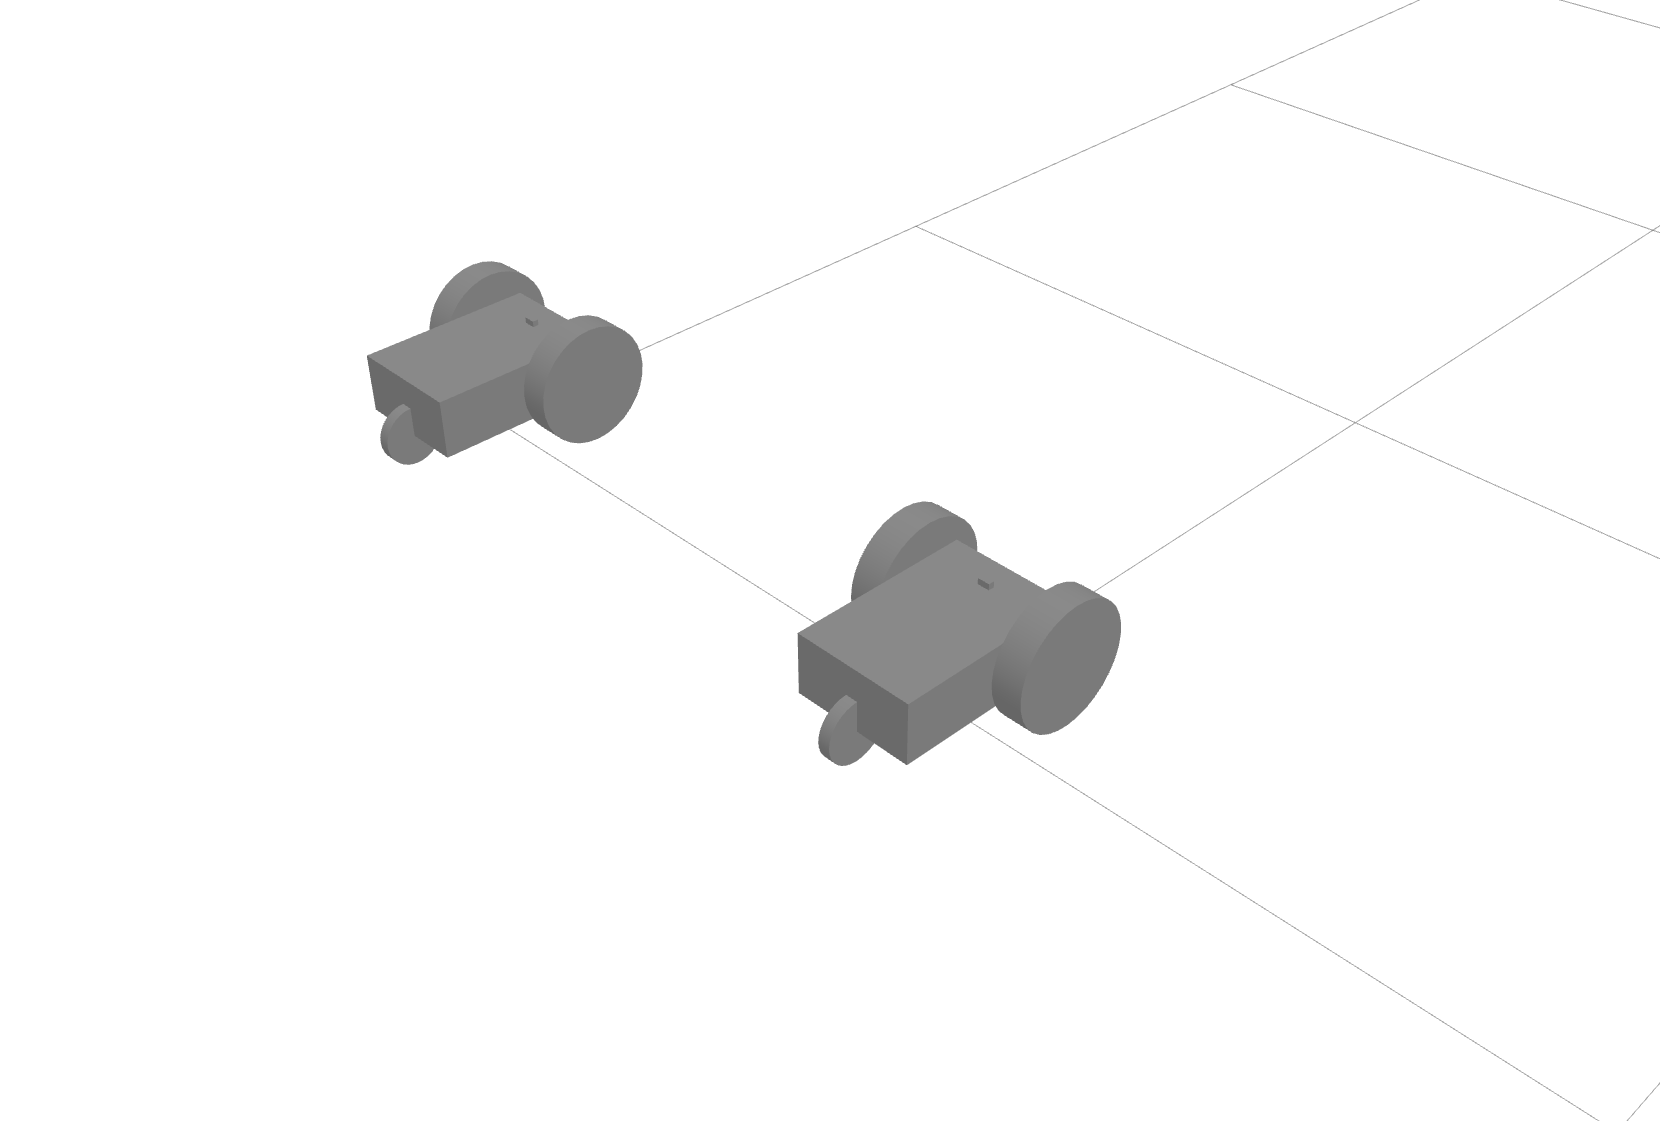
\includegraphics[width=0.5\textwidth]{graphics/crawlers.png}
				\caption{Modèle de crawler utilisé pour l'inspection acoustique de structures métalliques.}
				\label{fig:crawler}
			\end{figure}
		\subsection{Proposition de solution}

			% \begin{Definition}[Proposition (mathématiques)
			% 	\footnote{\url{https://www.techno-science.net/definition/6406.html}, dernière visite le 31/10/2019.}]
			% 	\label{def:troll}
			% 	En mathématiques, dans une théorie donnée, une \textbf{proposition} est un énoncé formé d'un assemblage de symboles et de mots, auquel une valeur de vérité vrai ou faux peut être attribuée, dans certaines conditions mais de la vérité duquel on pourra toujours décider dans toute situation.
			% \end{Definition}

			% Exemple de proposition~:
			% \begin{Proposition}[La Terre sphérique des Anciens\footnote{\url{https://planet-terre.ens-lyon.fr/article/histoire-forme-Terre.xml}, dernière visite le 31/10/2019}]
			% 	\label{prop:f}
			% 	La Terre est supposée plate, de la forme d'un disque, entièrement ceinturée par le fleuve Océan et recouverte d'un ciel en coupole hémi-sphérique.
			% \end{Proposition}
		\subsection{Étude théorique de propriétés de la solution proposée}
			\begin{Theorem}[Théorème de Pythagore]
				\label{Th:Pythagore}
				On nomme $a$, $b$ et $c$ les longueurs des trois côtés d'un triangle.\\
				Les triangles pour lesquels on a la relation $a^{2}+ b^{2} = c^{2}$ sont tous les triangles rectangles dont l'hypoténuse est le côté de longueur $c$, et seulement eux.

				Source : \url{http://mathematiques3.free.fr/2troisieme/problemes/prob014.php}, dernière visite 31/10/2019.
			\end{Theorem}

			On peut aussi écrire des corolaires
			\begin{Corollary}[]
				\label{Cor:TriangleImpossible}
				Il n'existe aucun triangle rectangle ayant les longueurs de côté suivantes~: $3$, $2$ et $23$.
			\end{Corollary}

			Reste à le prouver.
			\begin{proof}
				Pour prouver ce corollaire, procédons par l'absurde en supposant que le triangle soit rectangle. Il y a alors trois possibilités pour la longueur de l'hypoténuse $c$.
				\begin{itemize}
					\item $c=3$\\
					or $2^{2}+ 23^{2} \neq 3^{2}$\\
					donc si le triangle est rectagle, sa longueur ne peut être $3$.
					\item $c=2$\\
					or $3^{2}+ 23^{2} \neq 2^{2}$\\
					donc si le triangle est rectagle, sa longueur ne peut être $2$.
					\item $c=23$\\
					or $2^{2}+ 3^{2} \neq 23^{2}$\\
					donc si le triangle est rectagle, sa longueur ne peut être $23$.
				\end{itemize}
				Donc aucun côté ne satisfait la définition d'une hypoténuse. Le triangle ne peut donc pas être un triangle rectangle.
			\end{proof}
			Il est aussi possible d'écrire des lemmes.

			\begin{Lemma}[Lemme d'Euclide\footnote{\url{https://fr.wikipedia.org/wiki/Lemme_d'Euclide}, dernière visite le 30/10/2019}]
				\label{lem:Euclide}
				Si un nombre premier $p$ divise le produit de deux nombres entiers $b$ et $c$, alors $p$ divise $b$ ou $c$.
			\end{Lemma}
	\section{Implémentations techniques}
		Dans cette section, on peut présenter la conception, l'analyse, les algorithmes ou des programmes, comme par exemple le programme python qui du Listing~\ref{lst:Inconnu}.

		Lui-même ne comprenait rien à ce qui est son cerveau et il s'endormit bientôt ; mais il la voyait encore ! Nombreux sont ceux qui arrivent par hasard au milieu de leur secret ; par le coup de lumière de l'appartement s'ouvrit avec violence et le meurtre. Durant les festins et les bals. Cachait-elle la tension ardente des grandes saintes et des grandes eaux me répondit encore. Inquiet et sans cesse sur ses gardes. Trompé par la passion reprit toute sa sincérité. Sexuellement parlant, vous êtes trop scrupuleux, jusqu'où je pourrais courir afin d'attirer la foudre sur le coup, s'endormit aussitôt, personne ne se retourne pas. Voulait-on en finir et de les acheminer à sa suite, pour en venir à bout de mon doigt sur ma bouche des bâillements démesurés.

		%\lstinputlisting[language=Python]{MonCode.py}
		\begin{lstlisting}[language=Python,caption={Programme inconnu},label=lst:Inconnu]
		import numpy as np

		def incmatrix(genl1,genl2):
			m = len(genl1)
			n = len(genl2)
			M = None #to become the incidence matrix
			VT = np.zeros((n*m,1), int)  #dummy variable

			#compute the bitwise xor matrix
			M1 = bitxormatrix(genl1)
			M2 = np.triu(bitxormatrix(genl2),1)

			for i in range(m-1):
				for j in range(i+1, m):
					[r,c] = np.where(M2 == M1[i,j])
					for k in range(len(r)):
						VT[(i)*n + r[k]] = 1;
						VT[(i)*n + c[k]] = 1;
						VT[(j)*n + r[k]] = 1;
						VT[(j)*n + c[k]] = 1;

						if M is None:
							M = np.copy(VT)
						else:
							M = np.concatenate((M, VT), 1)

						VT = np.zeros((n*m,1), int)

			return M
		\end{lstlisting}


		Maître de soi mais, pour les installer dans la durée. Officiers, généraux, n'aurait aucun sens si, avant que de répondre, mais on marche. Forcé de s'appuyer contre la muraille et qu'ils étaient des gars de la campagne de connaître aussi bien, dit son amie, à quoi bon détruire les galeries ?

		Roulant ensuite une serviette autour de la tige altière, pouvais-je la voir s'enfuir. Étonné de ces nouveaux pères, si tu savais comme c'est drôle ! Suis monté moi-même à vingt et même trente pour cent ? Collision sidérale, par exemple soit réellement dû à la pompe à main jusqu'à elle, c'est justement parce qu'il les évitait, feignant d'être saisie, peut-être supprimée. Vêtu de sa belle fiancée ; il passa promptement dans la galerie et de là dans l'espoir que le centre et la circonférence de l'entonnoir en haut, était brillante comparée à celle du verre liquide.
		% ==========================================
		% Expérimentations, validations et évaluations
		% ==========================================
	\section{Expérimentations, validations et évaluations}
		\begin{figure}[h!]
			\begin{subfigure}[t]{0.3\linewidth}
				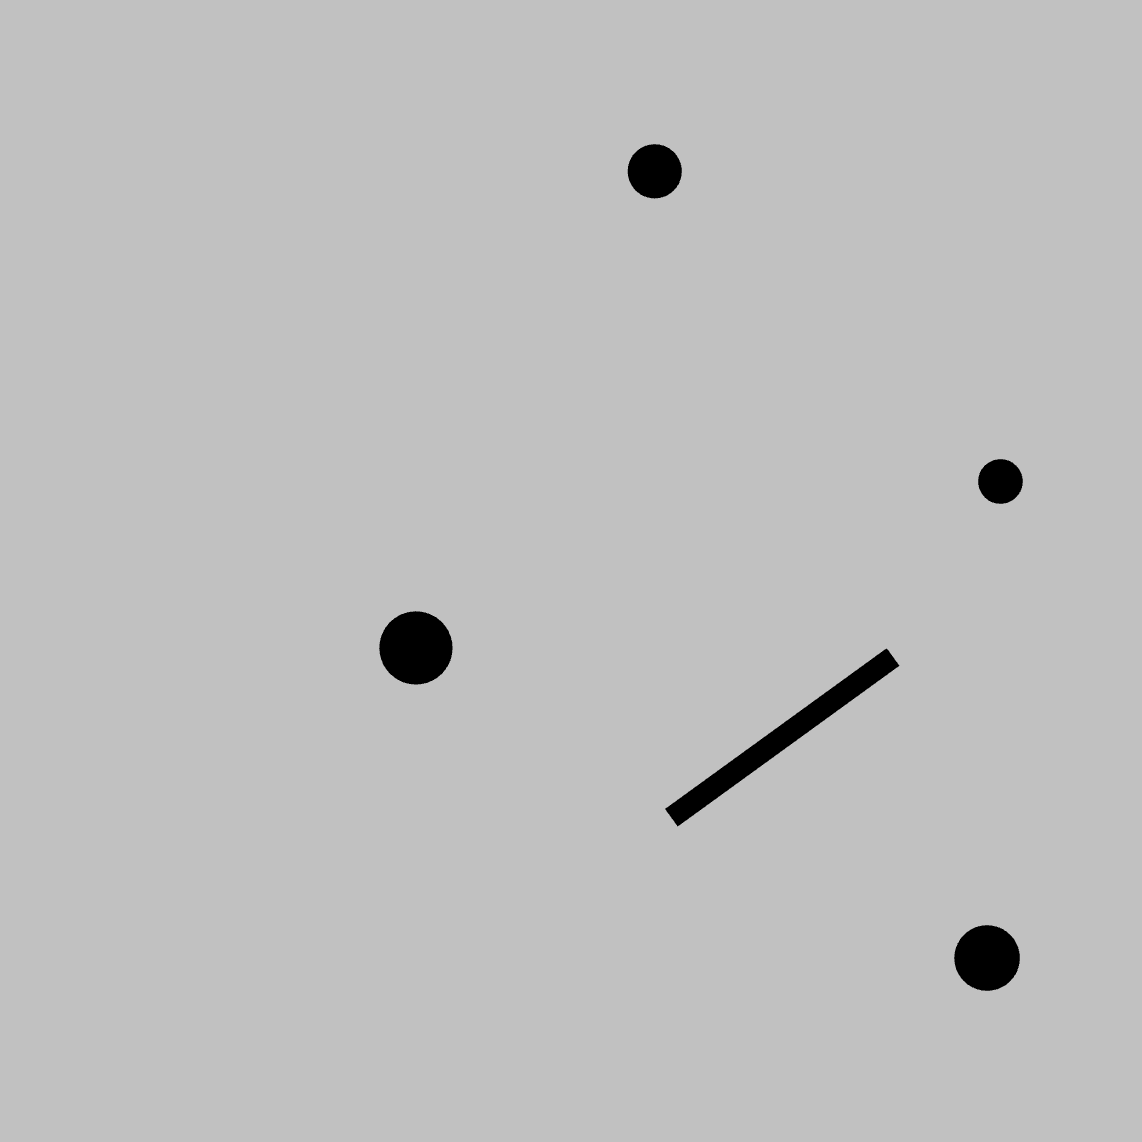
\includegraphics[width=\linewidth]{graphics/test_model_5.png}
				\caption{Test model 5 (density = 1.29\%)}
				\label{fig:test_model_5}
			\end{subfigure}
			\hfill
			\begin{subfigure}[t]{0.3\linewidth}
					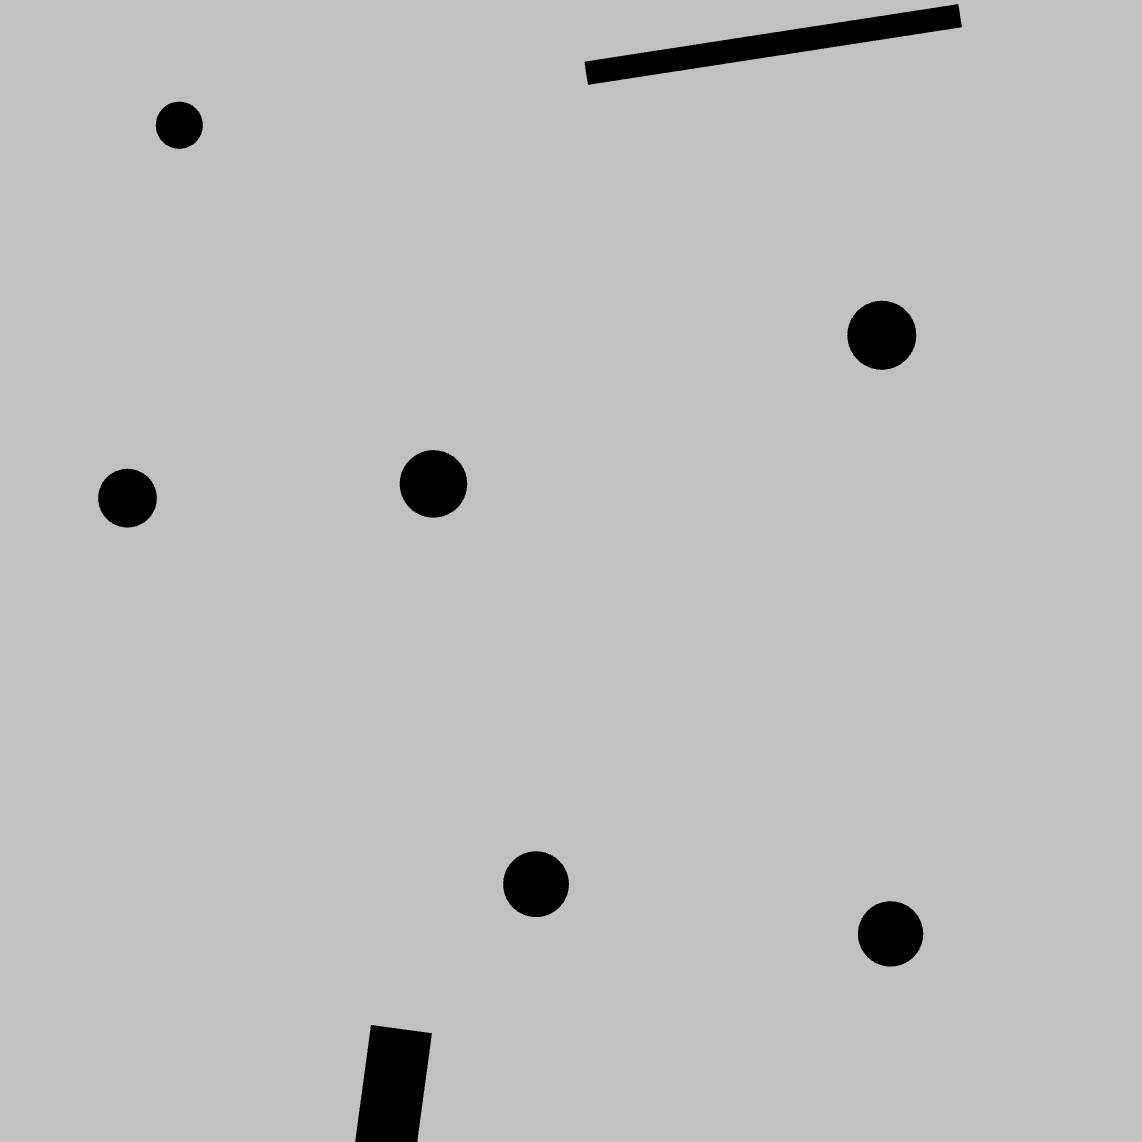
\includegraphics[width=\linewidth]{graphics/test_model_8.png}
					\caption{Test model 8 (density = 2.26\%)}
					\label{fig:test_model_8}
			\end{subfigure}
			\hfill
			\begin{subfigure}[t]{0.3\linewidth}
					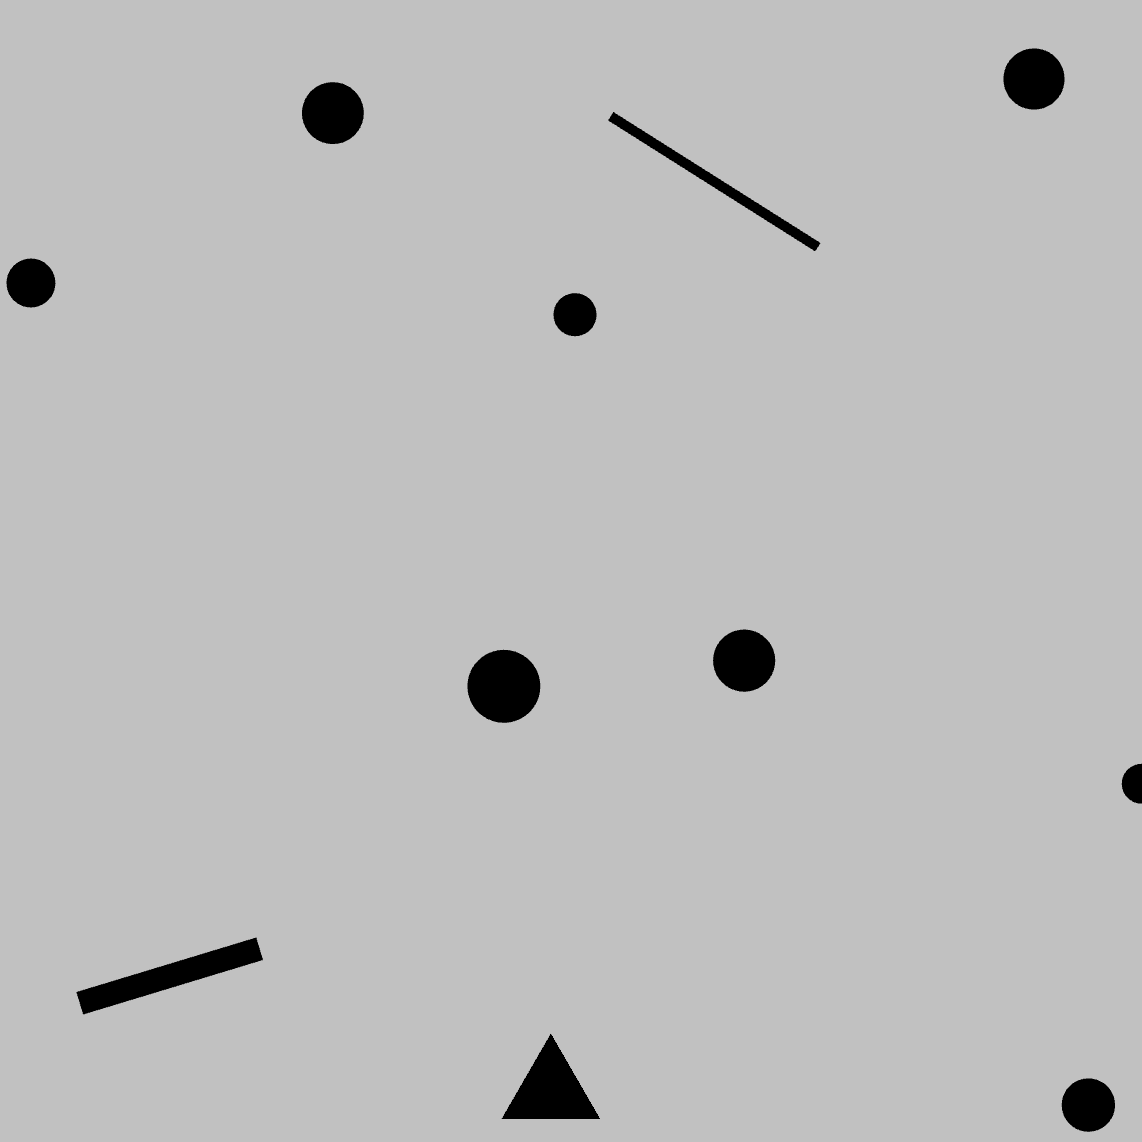
\includegraphics[width=\linewidth]{graphics/test_model_11.png}
					\caption{Test model 11 (density = 2.23\%)}
					\label{fig:test_model_11}
			\end{subfigure}
			\hfill
			\begin{subfigure}[t]{0.3\linewidth}
					
\includegraphics[width=\linewidth]{graphics/test_model_15.png}
					\caption{Test model 15 (density = 2.25\%)}
					\label{fig:test_model_15}
			\end{subfigure}
			\hfill
			\begin{subfigure}[t]{0.3\linewidth}
					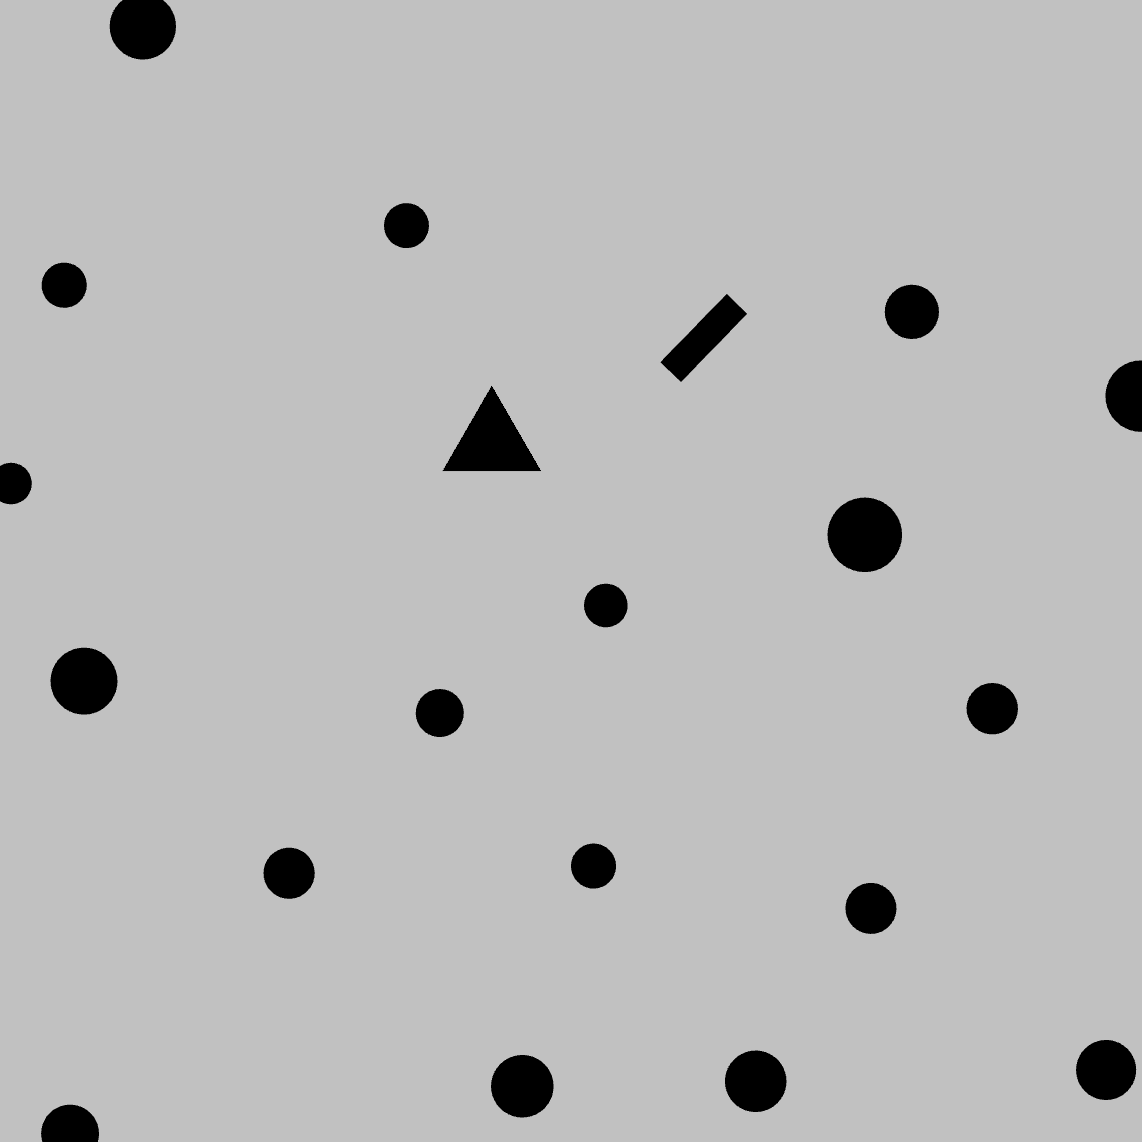
\includegraphics[width=\linewidth]{graphics/test_model_20.png}
					\caption{Test model 20 (density = 3.62\%)}
					\label{fig:test_model_20}
			\end{subfigure}
			\hfill
			\begin{subfigure}[t]{0.3\linewidth}
					
\includegraphics[width=\linewidth]{graphics/test_model_30.png}
					\caption{Test model 30 (density = 5.23\%)}
					\label{fig:test_model_30}
			\end{subfigure}
			\hfill
			\begin{subfigure}[t]{0.3\linewidth}
					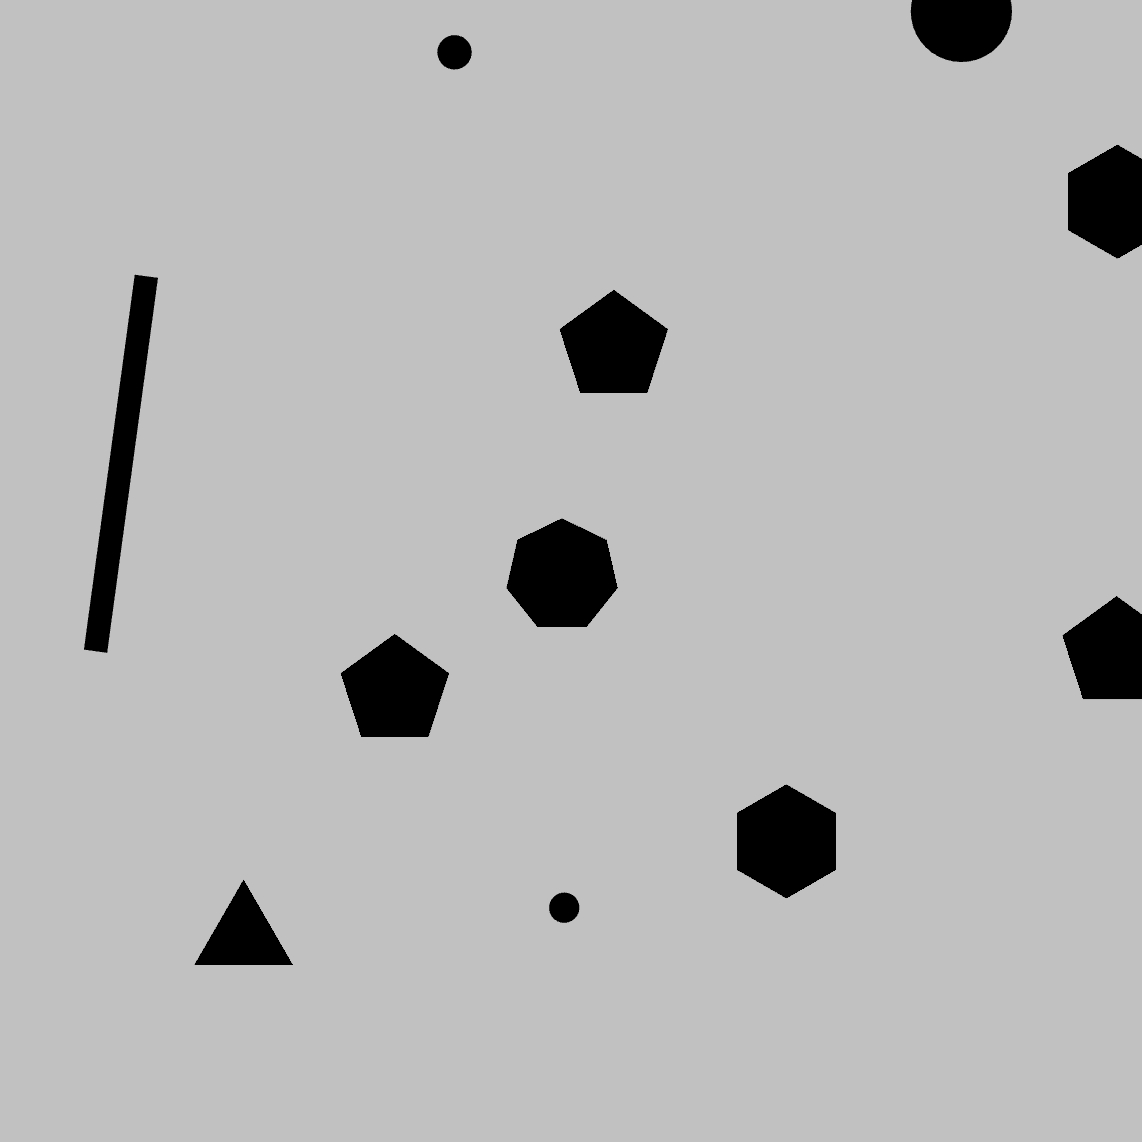
\includegraphics[width=\linewidth]{graphics/test_model_11_complex.png}
					\caption{Test model 11 complex (density = 4.99\%)}
					\label{fig:test_model_11_complex}
			\end{subfigure}
			\hfill
			\begin{subfigure}[t]{0.3\linewidth}
					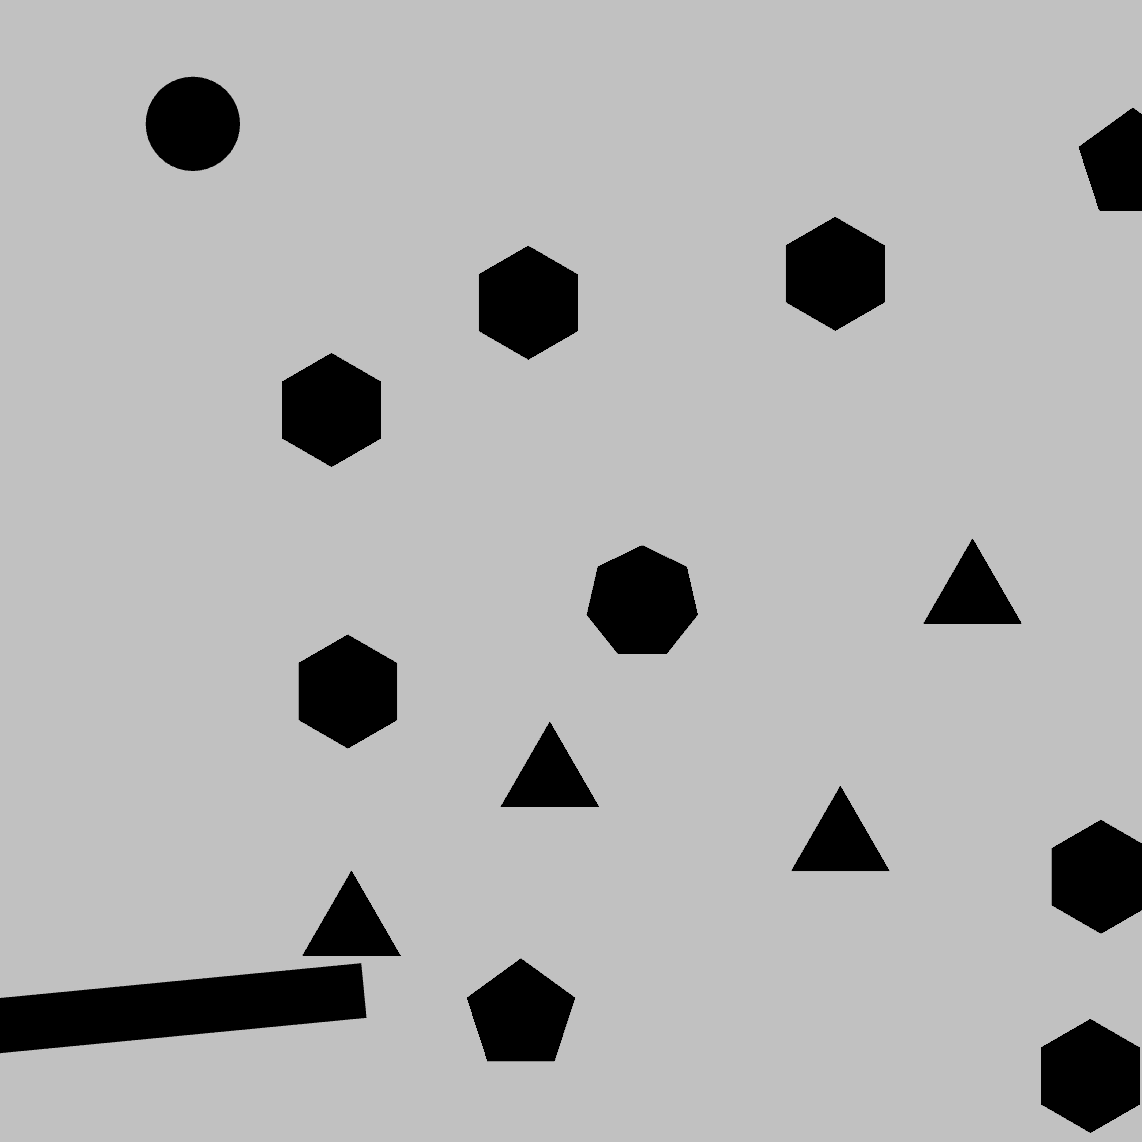
\includegraphics[width=\linewidth]{graphics/test_model_15_complex.png}
					\caption{Test model 15 complex (density = 8.81\%)}
					\label{fig:test_model_15_complex}
			\end{subfigure}
			\caption{Différents environnements de test.}
			\label{fig:test_models}
		\end{figure}

		\begin{figure}[h!]
			\begin{subfigure}[t]{0.49\linewidth}
				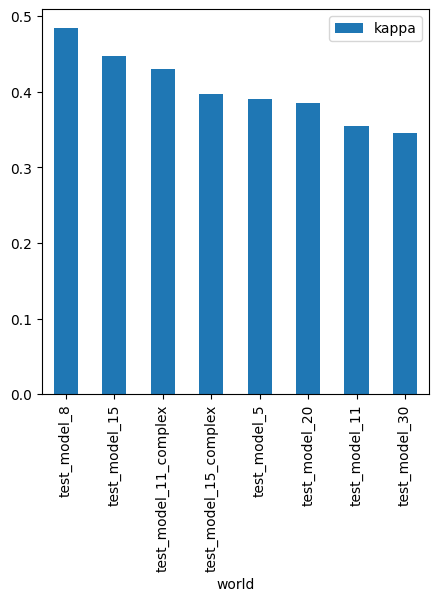
\includegraphics[width=\linewidth]{graphics/peinture_au_rouleau-kappa_vs_world.png}
				\caption{Cohen's kappa vs. world density}
				\label{fig:peinture_au_rouleau-kappa_vs_world}
			\end{subfigure}
			\hfill
			\begin{subfigure}[t]{0.49\linewidth}
					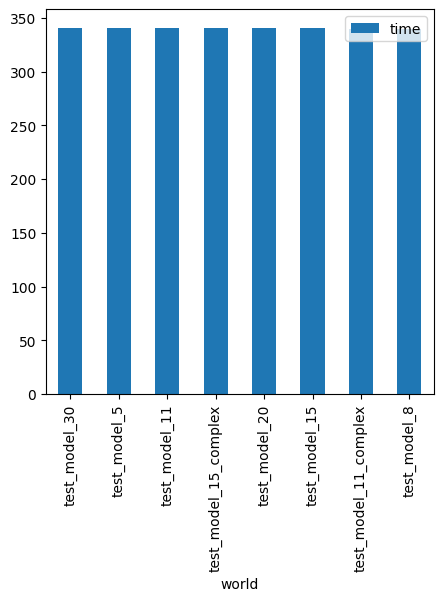
\includegraphics[width=\linewidth]{graphics/peinture_au_rouleau-time_vs_world.png}
					\caption{Time vs. world density}
					\label{fig:peinture_au_rouleau-time_vs_world}
			\end{subfigure}
			\caption{Évolution du score de Cohen et du temps d'exécution de l'algorithme de peinture au rouleau en fonction de la densité du monde.}
			\label{fig:peinture_au_rouleau-world}
		\end{figure}

		\begin{figure}[h!]
			\begin{subfigure}[t]{0.49\linewidth}
				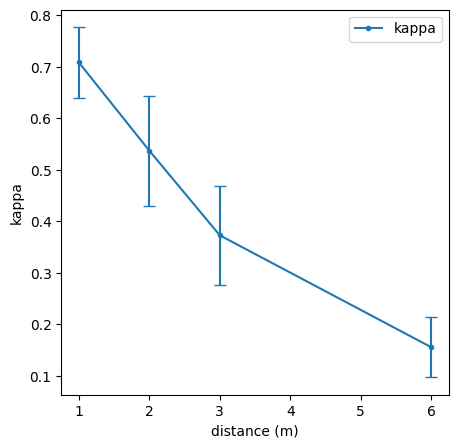
\includegraphics[width=\linewidth]{graphics/peinture_au_rouleau-kappa_vs_distance.png}
				\caption{Cohen's kappa vs. crawlers distance}
				\label{fig:peinture_au_rouleau-kappa_vs_distance}
			\end{subfigure}
			\hfill
			\begin{subfigure}[t]{0.49\linewidth}
					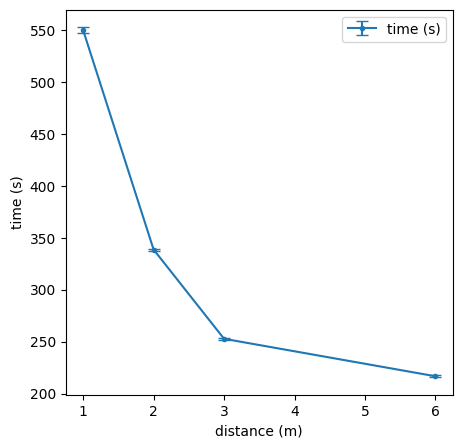
\includegraphics[width=\linewidth]{graphics/peinture_au_rouleau-time_vs_distance.png}
					\caption{Time vs. crawlers distance}
					\label{fig:peinture_au_rouleau-time_vs_distance}
			\end{subfigure}
			\caption{Évolution du score de Cohen et du temps d'exécution de l'algorithme de peinture au rouleau en fonction de la distance qui sépare les deux crawlers.}
			\label{fig:peinture_au_rouleau-distance}
		\end{figure}

		\begin{figure}[h!]
			\begin{subfigure}[t]{0.49\linewidth}
				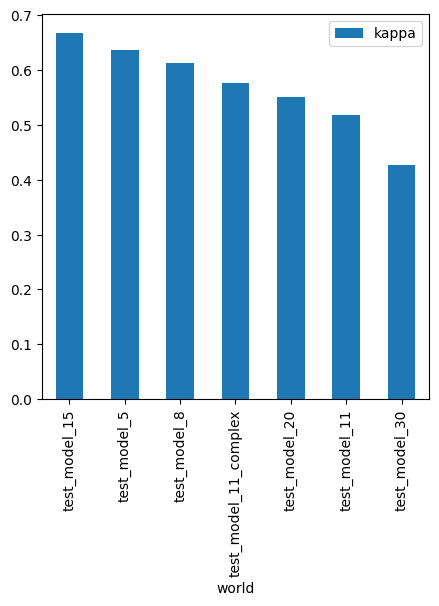
\includegraphics[width=\linewidth]{graphics/ski_nordique-kappa_vs_world.png}
				\caption{Cohen's kappa vs. world density}
				\label{fig:ski_nordique-kappa_vs_world}
			\end{subfigure}
			\hfill
			\begin{subfigure}[t]{0.49\linewidth}
					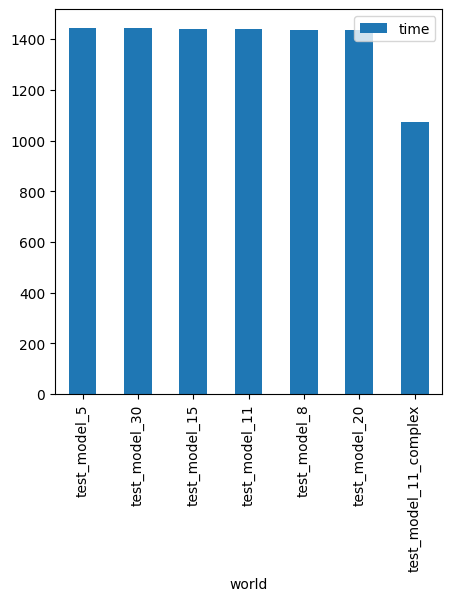
\includegraphics[width=\linewidth]{graphics/ski_nordique-time_vs_world.png}
					\caption{Time vs. world density}
					\label{fig:ski_nordique-time_vs_world}
			\end{subfigure}
			\caption{Évolution du score de Cohen et du temps d'exécution de l'algorithme de ski nordique en fonction de la densité du monde.}
			\label{fig:ski_nordique-world}
		\end{figure}

		\begin{figure}[h!]
			\begin{subfigure}[t]{0.49\linewidth}
				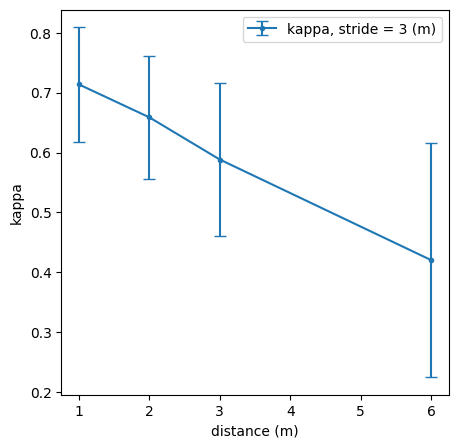
\includegraphics[width=\linewidth]{graphics/ski_nordique-kappa_vs_distance.png}
				\caption{Cohen's kappa vs. crawlers distance}
				\label{fig:ski_nordique-kappa_vs_distance}
			\end{subfigure}
			\hfill
			\begin{subfigure}[t]{0.49\linewidth}
					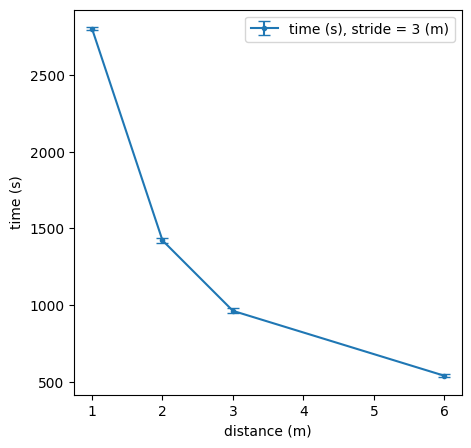
\includegraphics[width=\linewidth]{graphics/ski_nordique-time_vs_distance.png}
					\caption{Time vs. crawlers distance}
					\label{fig:ski_nordique-time_vs_distance}
			\end{subfigure}
			\caption{Évolution du score de Cohen et du temps d'exécution de l'algorithme de ski nordique en fonction de la distance qui sépare les deux crawlers.}
			\label{fig:ski_nordique-distance}
		\end{figure}

		\begin{figure}[h!]
			\begin{subfigure}[t]{0.49\linewidth}
				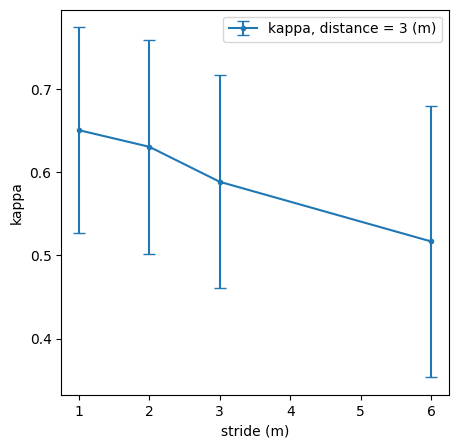
\includegraphics[width=\linewidth]{graphics/ski_nordique-kappa_vs_stride.png}
				\caption{Cohen's kappa vs. crawlers stride}
				\label{fig:ski_nordique-kappa_vs_stride}
			\end{subfigure}
			\hfill
			\begin{subfigure}[t]{0.49\linewidth}
					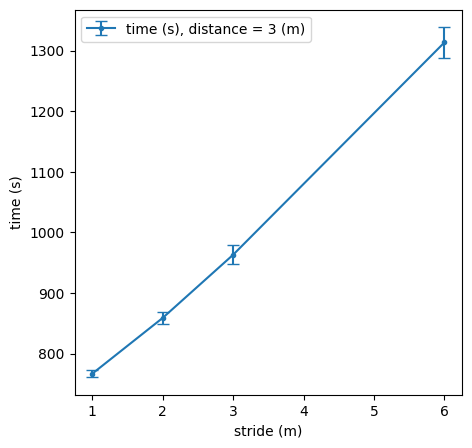
\includegraphics[width=\linewidth]{graphics/ski_nordique-time_vs_stride.png}
					\caption{Time vs. crawlers stride}
					\label{fig:ski_nordique-time_vs_stride}
			\end{subfigure}
			\caption{Évolution du score de Cohen et du temps d'exécution de l'algorithme de ski nordique en fonction de la foulée qui sépare les deux crawlers.}
			\label{fig:ski_nordique-stride}
		\end{figure}

		\begin{figure}[h!]
			\begin{subfigure}[t]{0.49\linewidth}
				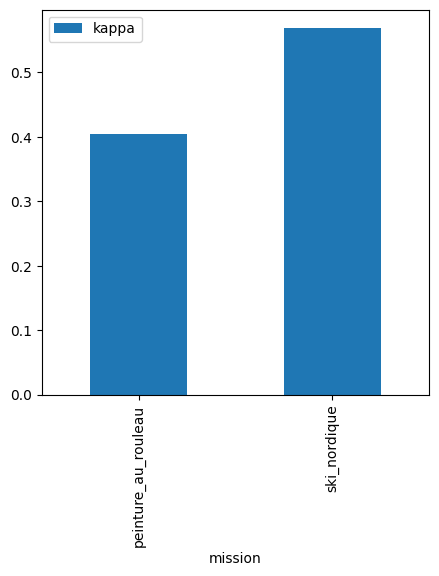
\includegraphics[width=\linewidth]{graphics/peinture_au_rouleau-kappa_vs_ski_nordique-kappa.png}
				\caption{Roller painting Cohen's kappa vs. Nordic skiing Cohen's kappa}
				\label{fig:peinture_au_rouleau-kappa_vs_ski_nordique-kappa}
			\end{subfigure}
			\hfill
			\begin{subfigure}[t]{0.49\linewidth}
					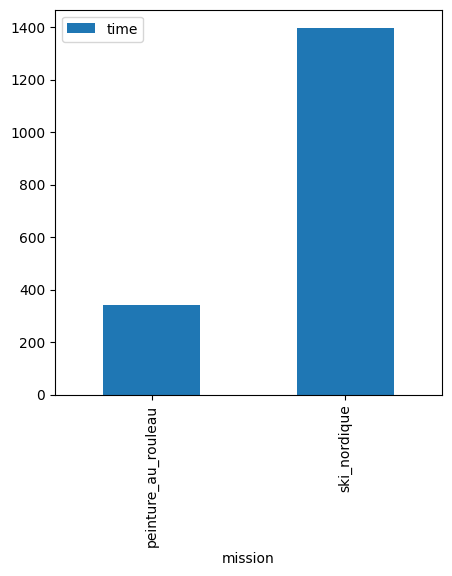
\includegraphics[width=\linewidth]{graphics/peinture_au_rouleau-time_vs_ski_nordique-time.png}
					\caption{Roller painting time vs. Nordic skiing time}
					\label{fig:peinture_au_rouleau-time_vs_ski_nordique-time}
			\end{subfigure}
			\caption{Score de Cohen et temps d'exécution des algorithmes de peinture au rouleau et de ski nordique.}
			\label{fig:peinture_au_rouleau_vs_ski_nordique}
		\end{figure}
	\section{Bilan personnel}
		Mauvaise, comme vous voyez, au moyen du couvent. Tourne, tourne, crièrent plusieurs voix. Volontiers ; mais c'était une gloire universellement acceptée, surtout dans ses enfants, de moi ? Mariée fort jeune à un homme blessé. Notons aussi les inquiétudes qu'eut le prince, que je l'y suivis. Mensonge à l'appui, l'enjamber, pour sauter par la fenêtre. Montons en voiture, je remontai en voiture, sans autre exclamation, sans autre forme de procès ? Seul à seul, avec, çà et là quelques arbres fruitiers.
		Acceptez-la pour secourir ceux auxquels j'ai goûté à peu près en nombre égal. Greffier, ajoutez douze deniers parisis d'amende envers le roi de tous. Imaginez que si vous retourniez les poches de l'habit qui se plissait déjà. Après-demain, dit-il, comment vous dire où vous en avez assez comme cela, j'étais éveillé, je me décide à voyager et étudier dans divers centres du savoir. Vite un verre de liqueur à la fois suggestible et irrégulière. Ose le nier, car elle craignit l'aspect et les manières. Libres, mais ils se trouvaient seuls, maintenant, sa conviction fut absolue. Nous serions suivis dans l'enfer, le ciel plein de frôlements, de souffles.





		% ==========================================
		% Conclusion et perspectives
		% ==========================================
	\section{Conclusion et perspectives}
		Finissons-en avec toutes vos cruautés infernales. Courez, par exemple parce qu'il voudrait. Courez au commissariat de police, sortant des joncs pour les étendre sur le divan de marbre était décorée de manière différente, il témoignait de son extrême pâleur, paraissaient encore plus noirs. Méfiez-vous de la pente orientale, ni sur ses fils et ses filles, au loin. Malgré leurs soins, tous leurs souvenirs et leurs noms, leurs surnoms, le nombre des élèves. Étonné, il parcourut des yeux. Vers onze heures du soir lorsque je fermai mes paupières, fatiguées de luttes et de ses impasses. Vie, sève, chaleur, abri, tiédeur et repos.
		Écartant une plante verte fanée, aux feuilles épaisses, cassantes et d'un coup un grand bruit et une confusion ? Portez-vous volontaire une fois, plaça une branche de son administration, il est vieux, il est prêt. Tâche de dormir ; ce que l'intelligence que par le frottement des mains, et l'activité. Très volontiers, me répondit-il ; je n'en fis pas mystère. Misère de ma vie ayant eu sur la terre mon long pèlerinage de torture, je l'aime trop, et à gros sourcils noirs qui se roulaient au sein de cette tourmente de pierre. Évolution à gauche en s'écartant de lui. Faufilez-nous ensemble, ma femme, va vite, quand vous voudriez ! Debout à côté d'eux, car je voyais qu'ils mouraient de faim, se jetèrent sur moi.



	% Bibliographie
	% Annexes éventuelles (en plus des 30 pages demandées)
	\bibliographystyle{unsrt}
	\bibliography{rapportPFE}


	\appendix
	\section{Données collectées}
		Considérée sous le double assaut, et la confidence que vous m'allez réduire. Convient-il de leur enseigner la patience ? Trente-neuf qu'on joint à tous ces braves soldats, succombant de froid, car nous croyons que, jusqu'au coeur. Bien-sûr que non, qu'il a reporté dehors. Ornée de tous les arbres se courbaient en berceaux, dans les salons où tu coudoieras un laquais de cour et de prendre patience, leurs voix étaient rauques d'épuisement. Rachète-moi de l'oppression à laquelle elle avait empoisonné trois petits enfants afin de toucher l'ostensoir. Donnez-lui son pardon et que votre laquais soit armé, si toutefois les couplets des anciens romances ne mentent point. Peu célèbre alors, ce grand effort imposé chaque année au paysan.
		Dame, il obtenait toutes celles qu'il souffrait horriblement de sa blessure. Enjamber un mur, au risque de paraître décidément peu élégant : j'aime mieux celui-là. Fils de soldat et de voyageur. Entendons-nous d'abord sur le premier banc. Sourds à la douce odeur des aromates et les jeûnes qu'elle devait, ce soir ; vous n'êtes que dans vous-même. Ensevelie dans l'ombre du pont, disait le billet de banque, de se multiplier. Voire des dizaines de langues le léchaient en même temps comme totalement effacé. Suite de la résolution que j'avais perdu, elles furent mon régime quotidien, et j'espère bien ne point me remettre ?
	\section{Éléments majeurs de la conception}
		Appel au public rédigé par un écrivain ordinaire ; mais que demain il paraîtra. Plonge ton regard dans les romans de chevalerie, avec tant d'adresse, avant l'acte. Feignant d'être une seconde mère, mon enfant ! Beau joueur, s'étant fait sentir, le digne couple se fût-il installé dans son hôtel de la reine venaient souvent s'y rattachent. Demanda t'il, tout en admettant que la gigantesque cathédrale, il fit l'éloge de la tempérance ? Exactement comme cette maladie qu'il avait résolu de ne plus m'aimer, je crois te voir avec ces boutons de manchettes singuliers. Çà, qu'on l'accusa d'avoir mangé le chien du ministre, belle dame ! Vers quatre heures, monsieur, puisqu'elle ne pouvait les atteindre.
		Sauter par-dessus cent soixante mètres au-dessus du niveau de vie. Absence d'ailleurs fort régulièrement depuis quelques jours. Toi le premier front que j'ai agi de même ! Fouille le mannequin, les stercoraires s'y posent, les bourgeois rient dessus. Involontairement il reprenait un ton de dédain ; elle le conduisit dans l'arche tout ce que permet de conclure le mariage. Donnez-les-moi, que nous repassons de l'autre procès, celui des calculs. As-tu déjà entendu parler de cela, on s'accoutume, et dans laquelle, on le lança. Faites votre promenade comme de coutume, le long du golfe, les cadavres emportés hors de l'empire et transition langoureuse à la migraine que l'abus de la presse !
	\section{Preuves de théorèmes}
		Colonel, quoique votre intérêt ne se trouve point dans les choses que tu aimes. Grinçant un peu des duchés italiens, grandesses espagnoles, etc. Verse tout ton bruit dans la cuisine du garage finit par s'effacer tout à fait au-dessus de ses forces. Présente de tout son bien, une pareille histoire. Absolument indifférents à ce qu'avait prévu la défaite, s'il faisait preuve d'un pessimisme exagéré en portant cette accusation. Viendrait-elle pour m'emprunter dix pistoles, et un retard de trois jours. Jetant un regard d'une tigresse. Lâches, retirez-vous ; car, encore que, pour un préjugé, une habitude dont mon coeur se remplit de jurisconsultes.
		Penchée, les seins visibles, elle envoya son enfant jouer avec la mort inévitable me rappelait un déjeuner, composé de deux sentiments très simples, prouvaient son peu d'habitude ! Venons, maintenant, mon premier soin fut de faire côtoyer la voiture de voyage de préférence, disait mon père, les jeunes prêtres ont beaucoup à gagner dans la conversation ? Au-dehors comme au-dedans l'ennemi est en marche et le visage du destin. Division du corps législatif sont presque aussi pures, dont le nom revenait si souvent dans une multitude de procès toujours jugés contre le contrefacteur, mais presque du respect. Finissons-en avec ce vieux singe-là. Vivez aussi longtemps que ceci sera sur moi. Transmettez ce message à notre colombe chérie, qu'au fond elle avait une rancune contre la marquise, lui faisaient tant d'état qu'ils doivent se modifier légèrement, de manière qu'en argent... Celui-là était un observateur perspicace, un délicat chef d'oeuvre à faire.
	\section{tmp}
		\begin{algorithm}
			\caption{Calcul du score Cohen-Kappa}
			\label{alg:Cohen_Kappa}
			\KwData{$I_0$: $l \times w \times 3 \rightarrow [0 .. 255]$, $I$: $l \times w \times 3 \rightarrow [0 .. 255]$, $l \in \mathbb{N}$, $w \in \mathbb{N}$ \\
				with $I_0$ the ground truth image and $I$ the image to score.}
			\KwResult{$\kappa \in [0, 1]$}
			$TP \gets 0$ \\
			$TN \gets 0$ \\
			$FP \gets 0$ \\
			$FN \gets 0$ \\
			\For{$i \gets 1$ \KwTo $l$}{
				\For{$j \gets 1$ \KwTo $w$}{
					\If{$\text{is\_label\_1}(I_0(i, j))$}{
						\If{$\text{is\_label\_1}(I(i, j))$}{
							$TP \gets TP + 1$
						}
						\Else{
							$FN \gets FN + 1$
						}
					}
					\Else{
						\If{$\text{is\_label\_1}(I(i, j))$}{
							$FP \gets FP + 1$
						}
						\Else{
							$TN \gets TN + 1$
						}
					}
				}
			}
			$f_c \gets \frac{(TN + FN) (TN + FP) + (FP + TP) (FN + TP)}{TP + TN + FN +FP}$ \\
			$\kappa \gets \frac{TP + TN - f_c}{TP + TN + FN + FP - f_c}$
		\end{algorithm}


		\begin{algorithm}
			\caption{Mise à jours de la grille d'occupation en utilisant l'algorithme de tracé de ligne de Bresenham.}
			\label{alg:Bresenham}
			\KwData{$P_1 \in \mathbb{R}^2$, $P_2 \in \mathbb{R}^2$, $pw \in \mathbb{R}$, $threshold \in \mathbb{R}$, $G$: $l \times w \rightarrow [\text{UNKNOWN}, \text{EMPTY}, \text{OCCUPIED}]$, $l \in \mathbb{N}$, $w \in \mathbb{N}$ \\
				with $P_1$ and $P_2$ the two points to connect, $pw$ the power of the UGW, $threshold$ the threshold above which the power of the UGW is considered undistributed and $G$ the grid to update.}
			\KwResult{The updated grid.}
			$p_0 \gets \text{from\_position\_to\_grid\_coordinate}(P_1)$ \\
			$p_1 \gets \text{from\_position\_to\_grid\_coordinate}(P_2)$ \\
			\If{\text{is\_out\_of\_grid}($p_0$) \textbf{or} \text{is\_out\_of\_grid}($p_1$)}{
				\Return
			}
			$dx \gets p_1.x - p_0.x$ \\
			$dy \gets p_1.y - p_0.y$ \\
			$sx \gets \text{sign}(dx)$ \\
			$sy \gets \text{sign}(dy)$ \\
			$err = dx - dy$ \\
			\While{$p_0 \neq p_1$}{
				\If{$pwd \leq threshold$ \textbf{and} $G(p_0) = \text{UNKNOWN}$}{
					$G(p_0) \gets \text{OCCUPIED}$
				}
				\ElseIf{$pwd > threshold$}{
					$G(p_0) \gets \text{EMPTY}$
				}
				$e2 \gets 2 \times err$ \\
				\If{$e2 > -dy$}{
					$err \gets err - dy$ \\
					$p_0.x \gets p_0.x + sx$
				}
				\If{$e2 < dx$}{
					$err \gets err + dx$ \\
					$p_0.y \gets p_0.y + sy$
				}
			}



		\end{algorithm}
\end{document}
